\documentclass[11pt,a4paper]{scrartcl}
\typearea{12}
\usepackage{graphicx}
\usepackage{pstricks}
\usepackage{listings}

\usepackage{tikz}
\usepackage{tikzscale}
\usepackage{pgfplots}

\usepackage{pgf}
\usepackage[utf8]{inputenc}
\usetikzlibrary{arrows,automata}
\usetikzlibrary{positioning}


\tikzset{
    state/.style={
           rectangle,
           rounded corners,
           draw=black, very thick,
           inner sep=2pt,
           text centered,
           },
}

\tikzset{
    stateon/.style={
           rectangle,
           rounded corners,
           draw=red, very thick,
           inner sep=2pt,
           text centered,
           fill=red!25,
           },
}


\tikzset{
    on/.style={
           circle,
           draw=red, very thick,
           inner sep=2pt,
           fill=red!25,
           },
}


\tikzset{
    off/.style={
           circle,
           draw=blue, very thick,
           inner sep=2pt,
           text centered,
           },
}


\pgfplotsset{compat=1.8}


\lstset{language=python}
\pagestyle{headings}
\markright{Computational Neuroscience - 10 neocortex}
\begin{document}

\subsection*{Introduction}
These notes are about memory in the neocortex; we will look at two
type of neocortical memory, recognition memory, which is believed to
occur in the perirhinal cortex, and the sort of long term memory which
is stored in what are called the association cortex, which is a
general term for that part of the neocortex that has no other name.



\subsection*{Memory}
We have looked at memory, medium term declarative memory, in the
specialized circuits that make up the hippocampus. This is only part
of memory, here we will briefly examine some other memory systems in
cortex, specifically, recognition memory and the way some declarative
memories are stored in cortex.

\subsection*{Recognition memory}

In situations where we might fail to name the items that make up the
contents of a room, we are often still able to spot a new or
unfamiliar item, an item that has been added since the room became
familiar to us. In fact, we are believed to have a separate system for
\textsl{recognition memory}: there was for some times a debate between
the idea that familiarity is a weak form of recognition, rather than a
separate type of memory, it is now believed that it is the latter,
with evidence from psychology \cite{Yonelinas2002a} and neuroscience
\cite{BrownAggleton2001a}. It is believed that recognition memory is
stored in the perirhinal cortex, an area of cortex immediately beside
the entorhinal cortex we discussed as part of the hippocampus.


Perhaps the most striking thing about recognition memory is its almost
limitless capacity, see Fig.~\ref{fig:standing}. This is thought to be
the consequence of the simpler task it performs, as illustrated in
Fig.~\ref{fig:recognition}, recognizing familiarity takes far fewer
connections than recalling a memory. In fact, we saw before that the
memory capacity for an auto-associative network such as that
attributed to CA3 is
\begin{equation}
P=\frac{0.035}{a}cN
\end{equation}
where $a$ is the sparseness, $c$ is the fraction of pairs that are
connected and $N$ is the number of neurons. The comparable formula for
a recognition network is
\begin{equation}
P=0.023cN^2.
\end{equation}
The $N^2$ rather than $N$ gives it a vastly larger capacity \cite{BogaczEtAl2001a}.

\begin{figure}
\begin{center}
% GNUPLOT: LaTeX picture with Postscript
\begingroup
  \makeatletter
  \providecommand\color[2][]{%
    \GenericError{(gnuplot) \space\space\space\@spaces}{%
      Package color not loaded in conjunction with
      terminal option `colourtext'%
    }{See the gnuplot documentation for explanation.%
    }{Either use 'blacktext' in gnuplot or load the package
      color.sty in LaTeX.}%
    \renewcommand\color[2][]{}%
  }%
  \providecommand\includegraphics[2][]{%
    \GenericError{(gnuplot) \space\space\space\@spaces}{%
      Package graphicx or graphics not loaded%
    }{See the gnuplot documentation for explanation.%
    }{The gnuplot epslatex terminal needs graphicx.sty or graphics.sty.}%
    \renewcommand\includegraphics[2][]{}%
  }%
  \providecommand\rotatebox[2]{#2}%
  \@ifundefined{ifGPcolor}{%
    \newif\ifGPcolor
    \GPcolorfalse
  }{}%
  \@ifundefined{ifGPblacktext}{%
    \newif\ifGPblacktext
    \GPblacktexttrue
  }{}%
  % define a \g@addto@macro without @ in the name:
  \let\gplgaddtomacro\g@addto@macro
  % define empty templates for all commands taking text:
  \gdef\gplbacktext{}%
  \gdef\gplfronttext{}%
  \makeatother
  \ifGPblacktext
    % no textcolor at all
    \def\colorrgb#1{}%
    \def\colorgray#1{}%
  \else
    % gray or color?
    \ifGPcolor
      \def\colorrgb#1{\color[rgb]{#1}}%
      \def\colorgray#1{\color[gray]{#1}}%
      \expandafter\def\csname LTw\endcsname{\color{white}}%
      \expandafter\def\csname LTb\endcsname{\color{black}}%
      \expandafter\def\csname LTa\endcsname{\color{black}}%
      \expandafter\def\csname LT0\endcsname{\color[rgb]{1,0,0}}%
      \expandafter\def\csname LT1\endcsname{\color[rgb]{0,1,0}}%
      \expandafter\def\csname LT2\endcsname{\color[rgb]{0,0,1}}%
      \expandafter\def\csname LT3\endcsname{\color[rgb]{1,0,1}}%
      \expandafter\def\csname LT4\endcsname{\color[rgb]{0,1,1}}%
      \expandafter\def\csname LT5\endcsname{\color[rgb]{1,1,0}}%
      \expandafter\def\csname LT6\endcsname{\color[rgb]{0,0,0}}%
      \expandafter\def\csname LT7\endcsname{\color[rgb]{1,0.3,0}}%
      \expandafter\def\csname LT8\endcsname{\color[rgb]{0.5,0.5,0.5}}%
    \else
      % gray
      \def\colorrgb#1{\color{black}}%
      \def\colorgray#1{\color[gray]{#1}}%
      \expandafter\def\csname LTw\endcsname{\color{white}}%
      \expandafter\def\csname LTb\endcsname{\color{black}}%
      \expandafter\def\csname LTa\endcsname{\color{black}}%
      \expandafter\def\csname LT0\endcsname{\color{black}}%
      \expandafter\def\csname LT1\endcsname{\color{black}}%
      \expandafter\def\csname LT2\endcsname{\color{black}}%
      \expandafter\def\csname LT3\endcsname{\color{black}}%
      \expandafter\def\csname LT4\endcsname{\color{black}}%
      \expandafter\def\csname LT5\endcsname{\color{black}}%
      \expandafter\def\csname LT6\endcsname{\color{black}}%
      \expandafter\def\csname LT7\endcsname{\color{black}}%
      \expandafter\def\csname LT8\endcsname{\color{black}}%
    \fi
  \fi
  \setlength{\unitlength}{0.0500bp}%
  \begin{picture}(5040.00,3528.00)%
    \gplgaddtomacro\gplbacktext{%
      \csname LTb\endcsname%
      \put(1210,704){\makebox(0,0)[r]{\strut{} 10}}%
      \put(1210,1557){\makebox(0,0)[r]{\strut{} 100}}%
      \put(1210,2410){\makebox(0,0)[r]{\strut{} 1000}}%
      \put(1210,3263){\makebox(0,0)[r]{\strut{} 10000}}%
      \put(1342,484){\makebox(0,0){\strut{} 10}}%
      \put(2442,484){\makebox(0,0){\strut{} 100}}%
      \put(3543,484){\makebox(0,0){\strut{} 1000}}%
      \put(4643,484){\makebox(0,0){\strut{} 10000}}%
      \put(176,1983){\rotatebox{-270}{\makebox(0,0){\strut{}$M$}}}%
      \put(2992,154){\makebox(0,0){\strut{}$S$}}%
    }%
    \gplgaddtomacro\gplfronttext{%
    }%
    \gplbacktext
    \put(0,0){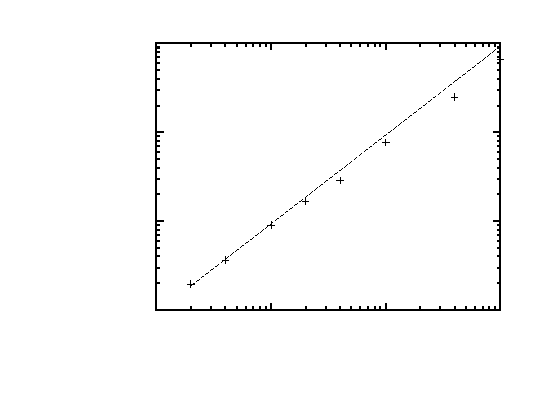
\includegraphics{standing}}%
    \gplfronttext
  \end{picture}%
\endgroup

\end{center}
\caption{Recognized images plotted against presented images. $S$ is the number of images presented, $M$ the number recognized as familiar in a forced-choice task. The data points are plotted from data presented in \cite{Standing1973a} and the line represents $\log_{10}{M}=0.93\log_{10}{S}+0.08$.\label{fig:standing}.}
\end{figure}

\begin{figure}
\textbf{A}
\begin{center}
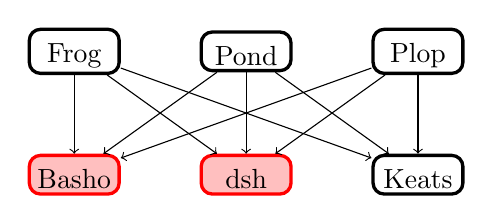
\begin{tikzpicture}
\node[state,text width=1cm, text height=0.35cm](0){Frog};
\node[state,text width=1cm, text height=0.35cm, right = 1cm of 0](1){Pond};
\node[state,text width=1cm, text height=0.35cm, right = 1cm of 1](2){Plop};
\node[stateon,text width=1cm, text height=0.35cm, below = 1cm of 0](3){Basho};
\node[stateon,text width=1cm, text height=0.35cm, right = 1cm of 3](4){dsh};
\node[state,text width=1cm, text height=0.35cm, right = 1cm of 4](5){Keats};
\path (0) edge[->] (3);
\path (0)  edge[->] (4);
\path (0) edge[->]  (5);
\path (1) edge[->]  (3);
\path (1) edge[->]  (4);
\path (1) edge[->]  (5);
\path (2) edge[->]  (3);
\path (2) edge[->]  (4);
\path (2) edge[->]  (5);
\end{tikzpicture}
\end{center}
\textbf{B}
\begin{center}
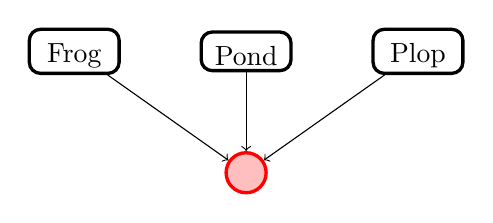
\begin{tikzpicture}
\node[state,text width=1cm, text height=0.35cm](0){Frog};
\node[state,text width=1cm, text height=0.35cm, right = 1cm of 0](1){Pond};
\node[state,text width=1cm, text height=0.35cm, right = 1cm of 1](2){Plop};
\node[on,text width=0.35cm,below = 1cm of 1](3){};
\path (0) edge[->] (3);
\path (1) edge[->]  (3);
\path (2) edge[->]  (3);
\end{tikzpicture}
\end{center}
\caption{Recognition circuits are simpler. In \textbf{A} is a schematic for recognizing dsh's translation of Matsuo Basho's haiku, with different nodes for the different concepts and, as a consequence, a large number of connections. In contrast, in \textbf{B} the goal is just to recognize the poem as familiar, so there is one familiarity neuron and far fewer connections.\label{fig:recognition}}
\end{figure}

This doesn't resolve how recognition is done; in fact there is a
diversity of approaches used. One interesting application is found in
\cite{BaddeleyEtAl2012a} where recognition memory is used as a
mechanism for visual navigation in ants. It is likely that any memory
is stored using a small subset of its features.

\subsection*{Declarative memories stored in cortex}

We have already examined the way declarative memories are stored in
the hippocampus; there are also declarative memories stored in cortex,
but, it seems, the cortical memories are stored in a different
way. While the hippocampus seems capable of storing memories very
quickly with little chance of overlap, the cortex appears to learn
memories slowly, in a way that discovers overlaps and exploits them
for learning. The idea is that memories are first stored in
hippocampus and, over time, if they are important, they are learnt
from their to neocortex, where they are stored in a rich,
interconnected, way.

Consider a simple model neuron with output
\begin{equation}
x_i=\sum w_{ij}x_j
\end{equation}
where $w_{ij}$ are connection strengths. Now the perceptron learning rule is
\begin{equation}
\Delta w_{ij}=\eta(h_i-x_i)x_j
\end{equation}
where $h_i$ is the desired output and $x_i$ the actual output. With
small $\eta$ this should converge over time to give $h_i=x_i$. The key here is that $\eta$ is small, so convergence is slow. Consider learning a series of birds\\[0.75cm]

\begin{tikzpicture}
\node[on,text width=0.35cm](0){};
\node[on,text width=0.35cm,right of = 0](1){};
\node[off,text width=0.35cm,right of = 1](2){};
\node[on,text width=0.35cm,right of = 2](3){};
\node[off,text width=0.35cm,right of = 3](4){};
\node[on,text width=0.35cm,right of = 4](5){};
\node[off,text width=0.35cm,right of = 5](6){};
\node[off,text width=0.35cm,right of = 6](7){};
\node[off,text width=0.35cm,right of = 7](8){};
\node[right of =8](bird){eagle};
\end{tikzpicture}\\

\begin{tikzpicture}
\node[on,text width=0.35cm](0){};
\node[on,text width=0.35cm,right of = 0](1){};
\node[off,text width=0.35cm,right of = 1](2){};
\node[on,text width=0.35cm,right of = 2](3){};
\node[off,text width=0.35cm,right of = 3](4){};
\node[off,text width=0.35cm,right of = 4](5){};
\node[on,text width=0.35cm,right of = 5](6){};
\node[off,text width=0.35cm,right of = 6](7){};
\node[off,text width=0.35cm,right of = 7](8){};
\node[right of =8](bird){wren};
\end{tikzpicture}\\

\begin{tikzpicture}
\node[on,text width=0.35cm](0){};
\node[on,text width=0.35cm,right of = 0](1){};
\node[off,text width=0.35cm,right of = 1](2){};
\node[on,text width=0.35cm,right of = 2](3){};
\node[off,text width=0.35cm,right of = 3](4){};
\node[off,text width=0.35cm,right of = 4](5){};
\node[off,text width=0.35cm,right of = 5](6){};
\node[on,text width=0.35cm,right of = 6](7){};
\node[off,text width=0.35cm,right of = 7](8){};
\node[right of =8](bird){parrot};
\end{tikzpicture}\\[0.5cm]
This is the sort of disastrous correlation we discussed in the
hippocampal context, hypothesising that random connections related to
neurogenisis are employed to lift the degeneracy. Here, however, it
allows properties to be deduced and stored.\\[0.75cm]
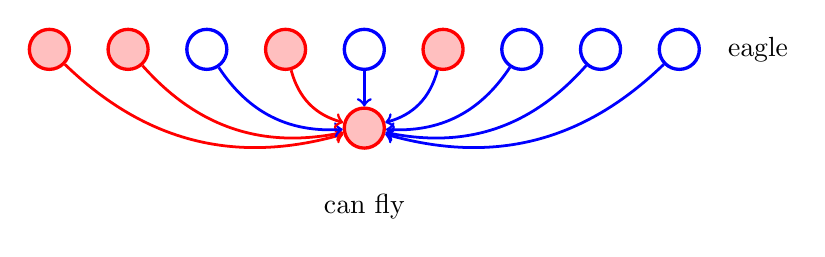
\begin{tikzpicture}
\node[on,text width=0.35cm](0){};
\node[on,text width=0.35cm,right of = 0](1){};
\node[off,text width=0.35cm,right of = 1](2){};
\node[on,text width=0.35cm,right of = 2](3){};
\node[off,text width=0.35cm,right of = 3](4){};
\node[on,text width=0.35cm,right of = 4](5){};
\node[off,text width=0.35cm,right of = 5](6){};
\node[off,text width=0.35cm,right of = 6](7){};
\node[off,text width=0.35cm,right of = 7](8){};
\node[right of =8](bird){eagle};
\node[on,text width=0.35cm, below of =4](9){};
\node[below of =9](fly){can fly};
\path (0) edge[->,red,line width=1pt, bend right] (9); 
\path (1) edge[->,red,line width=1pt, bend right] (9); 
\path (2) edge[->,blue,line width=1pt, bend right] (9); 
\path (3) edge[->,red,line width=1pt, bend right] (9); 
\path (4) edge[->,blue,line width=1pt] (9); 
\path (5) edge[->,blue,line width=1pt, bend left] (9); 
\path (6) edge[->,blue,line width=1pt, bend left] (9); 
\path (7) edge[->,blue,line width=1pt, bend left] (9); 
\path (8) edge[->,blue,line width=1pt, bend left] (9); 
\end{tikzpicture}\\[0.5cm]
The problem is that if a new bird is stored, this might lead to an erroneous conclusion\\[0.75cm]
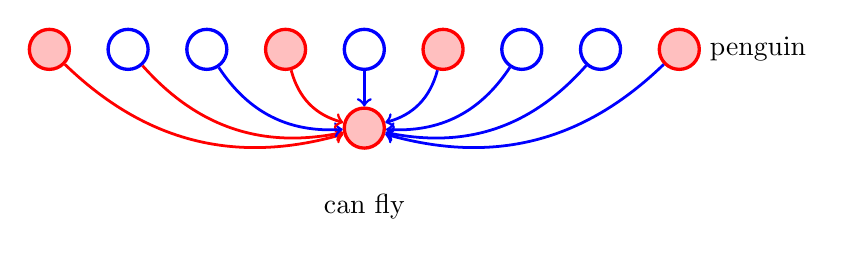
\begin{tikzpicture}
\node[on,text width=0.35cm](0){};
\node[off,text width=0.35cm,right of = 0](1){};
\node[off,text width=0.35cm,right of = 1](2){};
\node[on,text width=0.35cm,right of = 2](3){};
\node[off,text width=0.35cm,right of = 3](4){};
\node[on,text width=0.35cm,right of = 4](5){};
\node[off,text width=0.35cm,right of = 5](6){};
\node[off,text width=0.35cm,right of = 6](7){};
\node[on,text width=0.35cm,right of = 7](8){};
\node[right of =8](bird){penguin};
\node[on,text width=0.35cm, below of =4](9){};
\node[below of =9](fly){can fly};
\path (0) edge[->,red,line width=1pt, bend right] (9); 
\path (1) edge[->,red,line width=1pt, bend right] (9); 
\path (2) edge[->,blue,line width=1pt, bend right] (9); 
\path (3) edge[->,red,line width=1pt, bend right] (9); 
\path (4) edge[->,blue,line width=1pt] (9); 
\path (5) edge[->,blue,line width=1pt, bend left] (9); 
\path (6) edge[->,blue,line width=1pt, bend left] (9); 
\path (7) edge[->,blue,line width=1pt, bend left] (9); 
\path (8) edge[->,blue,line width=1pt, bend left] (9); 
\end{tikzpicture}\\[0.5cm]
However, if the sequences are presented enough times and the learning rate is low enough, the perceptron should be able to store the correct information
\\[0.75cm]
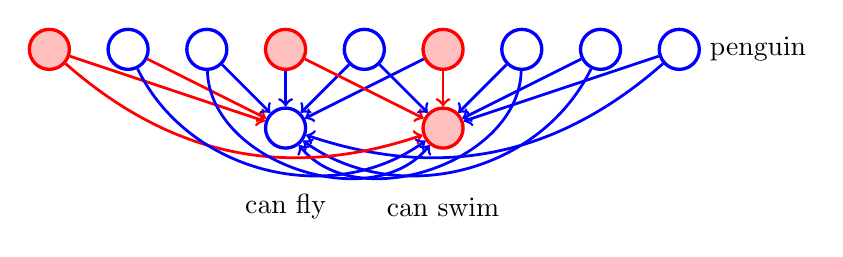
\begin{tikzpicture}
\node[on,text width=0.35cm](0){};
\node[off,text width=0.35cm,right of = 0](1){};
\node[off,text width=0.35cm,right of = 1](2){};
\node[on,text width=0.35cm,right of = 2](3){};
\node[off,text width=0.35cm,right of = 3](4){};
\node[on,text width=0.35cm,right of = 4](5){};
\node[off,text width=0.35cm,right of = 5](6){};
\node[off,text width=0.35cm,right of = 6](7){};
\node[off,text width=0.35cm,right of = 7](8){};
\node[right of =8](bird){penguin};
\node[off,text width=0.35cm, below of =3](9){};
\node[below of =9](fly){can fly};
\path (0) edge[->,red,line width=1pt] (9); 
\path (1) edge[->,red,line width=1pt] (9); 
\path (2) edge[->,blue,line width=1pt] (9); 
\path (3) edge[->,blue,line width=1pt] (9); 
\path (4) edge[->,blue,line width=1pt] (9); 
\path (5) edge[->,blue,line width=1pt] (9); 
\path (6) edge[->,blue,line width=1pt, bend left=70] (9); 
\path (7) edge[->,blue,line width=1pt, bend left=50] (9); 
\path (8) edge[->,blue,line width=1pt, bend left] (9); 
\node[on,text width=0.35cm, below of =5](10){};
\node[below of =10](fly){can swim};
\path (0) edge[->,red,line width=1pt, bend right] (10); 
\path (1) edge[->,blue,line width=1pt, bend right=50] (10); 
\path (2) edge[->,blue,line width=1pt, bend right=70] (10); 
\path (3) edge[->,red,line width=1pt] (10); 
\path (4) edge[->,blue,line width=1pt] (10); 
\path (5) edge[->,red,line width=1pt] (10); 
\path (6) edge[->,blue,line width=1pt] (10); 
\path (7) edge[->,blue,line width=1pt] (10); 
\path (8) edge[->,blue,line width=1pt] (10); 
\end{tikzpicture}\\[0.5cm]
but\\[0.75cm]
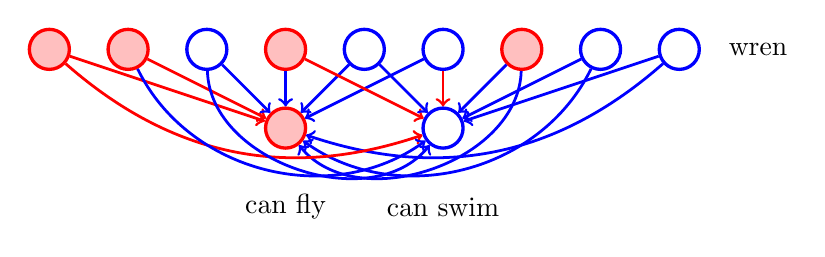
\begin{tikzpicture}
\node[on,text width=0.35cm](0){};
\node[on,text width=0.35cm,right of = 0](1){};
\node[off,text width=0.35cm,right of = 1](2){};
\node[on,text width=0.35cm,right of = 2](3){};
\node[off,text width=0.35cm,right of = 3](4){};
\node[off,text width=0.35cm,right of = 4](5){};
\node[on,text width=0.35cm,right of = 5](6){};
\node[off,text width=0.35cm,right of = 6](7){};
\node[off,text width=0.35cm,right of = 7](8){};
\node[right of =8](bird){wren};
\node[on,text width=0.35cm, below of =3](9){};
\node[below of =9](fly){can fly};
\path (0) edge[->,red,line width=1pt] (9); 
\path (1) edge[->,red,line width=1pt] (9); 
\path (2) edge[->,blue,line width=1pt] (9); 
\path (3) edge[->,blue,line width=1pt] (9); 
\path (4) edge[->,blue,line width=1pt] (9); 
\path (5) edge[->,blue,line width=1pt] (9); 
\path (6) edge[->,blue,line width=1pt, bend left=70] (9); 
\path (7) edge[->,blue,line width=1pt, bend left=50] (9); 
\path (8) edge[->,blue,line width=1pt, bend left] (9); 
\node[off,text width=0.35cm, below of =5](10){};
\node[below of =10](fly){can swim};
\path (0) edge[->,red,line width=1pt, bend right] (10); 
\path (1) edge[->,blue,line width=1pt, bend right=50] (10); 
\path (2) edge[->,blue,line width=1pt, bend right=70] (10); 
\path (3) edge[->,red,line width=1pt] (10); 
\path (4) edge[->,blue,line width=1pt] (10); 
\path (5) edge[->,red,line width=1pt] (10); 
\path (6) edge[->,blue,line width=1pt] (10); 
\path (7) edge[->,blue,line width=1pt] (10); 
\path (8) edge[->,blue,line width=1pt] (10); 
\end{tikzpicture}

In this way hippocampus and neocortex are thought to solve different
memory problems, a helpful analogy is given in
\cite{McClellandEtAl1995a}: imagine you drive to work each day, the
hippocampus would store the location of where you parked that morning
so you could get back to your car in the evening, your neocortex would
learn which places are good for parking.

\begin{thebibliography}{10}

\bibitem{Yonelinas2002a}
Yonelinas AP. (2002) The nature of recollection and familiarity: A
review of 30 years of research. 
\newblock Journal Memory and Language. 46: 441--571.

\bibitem{BrownAggleton2001a}
Brown MW and Aggleton JP. (2001) Recognition memory: What are the
roles of the perirhinal cortex and hippocampus. 
\newblock Nature Review Neuroscience. 2: 51--6

\bibitem{Standing1973a}
Standing L. (1973) Learning 10000 pictures.
\newblock  The Quarterly Journal of Experimental Psychology. 25: 207--22.

\bibitem{BogaczEtAl2001a}
Bogacz R, Brown MW and Giraud-Carrier C. (2001) Model of familiarity discrimination in the perirhinal cortex.
\newblock Journal of Computational Neuroscience. 10: 5--23.

\bibitem{BaddeleyEtAl2012a}
Baddeley B, Graham P, Husbands P and Philippides A (2012) A model of ant route navigation driven by scene familiarity. 
\newblock PLoS Computational Biology. 8: e1002336.

\bibitem{McClellandEtAl1995a}
McClelland JL, McNaughton BL and O'Reilly RC. (1995) Why there are complementary learning systems in the hippocampus and neocortex: insights from the successes and failures of connectionist models of learning and memory.
\newblock Psychological Review 102: 419.

\end{thebibliography}

\end{document}
